\subsection{Demostración de punta a punta}\label{sec:demo}
Con 300\,000 eventos (\texttt{scripts/demo.py}, salida completa en \texttt{docs/demo\_output.txt}) el pipeline procesa el stream a $\sim$12\,000 eventos/s;
con 1M eventos, a 7\,600 eventos/s, y con 10M, a 7\,674 eventos/s (Tabla~\ref{tab:pipe}). Ejemplos de recorridos registrados por el trazador:
(i) una \textbf{compra express} entra en la FIFO, E1 la valida y verifica por búsqueda binaria que no es duplicada, E2 la inserta con prioridad 2 y sale del heap sin
esperar, E3 la enriquece (producto, precio), E4 indexa su orden en el B+Tree, E6 la aprueba, E7 la usa en los conjuntos de compradores, E8 la incorpora al grafo de la
ventana y E9 devuelve un Top-5 para el usuario; (ii) un \textbf{intento de pago} de una ráfaga supera el umbral del CMS, se bloquea y la alerta re-inyectada se atiende
con prioridad 0; (iii) un registro con precio negativo se rechaza en E1 y una re-entrega duplicada se elimina en E1. En ningún tamaño los pagos, alertas o compras
esperaron en el heap (0 \emph{ticks}); solo las vistas/búsquedas esperaron en los picos (0.47–0.66 \emph{ticks} en promedio). Los positivos del Bloom se
verificaron en la tabla hash antes de bloquear: 0 bloqueos erróneos.

\begin{table}[H]\centering\small
\caption{Pipeline completo (20\,000 productos, micro-lote 5\,000; 10\,000 en 10M). Costo por etapa en µs por elemento que la etapa procesa.}\label{tab:pipe}
\resizebox{\linewidth}{!}{\setlength{\tabcolsep}{4pt}
\begin{tabular}{@{}rrrrrrrrrrrrrr@{}}\toprule
Eventos & Procesados & s & ev/s & RSS GB & Órd. aprob./bloq. & Alertas & E0 & E1 & E2 & E3 & E4 & E5 & E6 \\\midrule
$10^4$ & 9\,996 & 1 & 10\,333 & 0.1 & 348 / 2 & 3 & 10 & 4 & 5 & 5 & 4 & 56 & 91 \\
$10^5$ & 99\,901 & 9 & 11\,551 & 0.2 & 3\,480 / 17 & 3 & 5 & 5 & 5 & 5 & 4 & 37 & 99 \\
$10^6$ & 999\,061 & 132 & 7\,597 & 1.1 & 34\,808 / 146 & 20 & 7 & 15 & 7 & 7 & 5 & 37 & 78 \\
$10^7$ & 9\,990\,165 & 1302 & 7\,674 & 4.5 & 348\,074 / 1405 & 200 & 15 & 15 & 11 & 10 & 5 & 38 & 63 \\
\bottomrule\end{tabular}}
\end{table}
\vspace{-6pt}
La etapa más costosa por elemento es E7 (reconstrucción del LSH y, sobre todo, la construcción del HNSW de 20\,000 productos, 40\,s fijos de inicialización), seguida
por E6 (Bloom + dos CMS escalares por pago, 63–99\,µs) y E5 (KD-Tree, $\sim$37\,µs, mitigado por un LRU con 69\,\% de aciertos). E0–E4 cuestan 4–15\,µs por evento.

\subsection{Estructuras base (E0–E5, E9)}
\begin{figure}[H]\centering
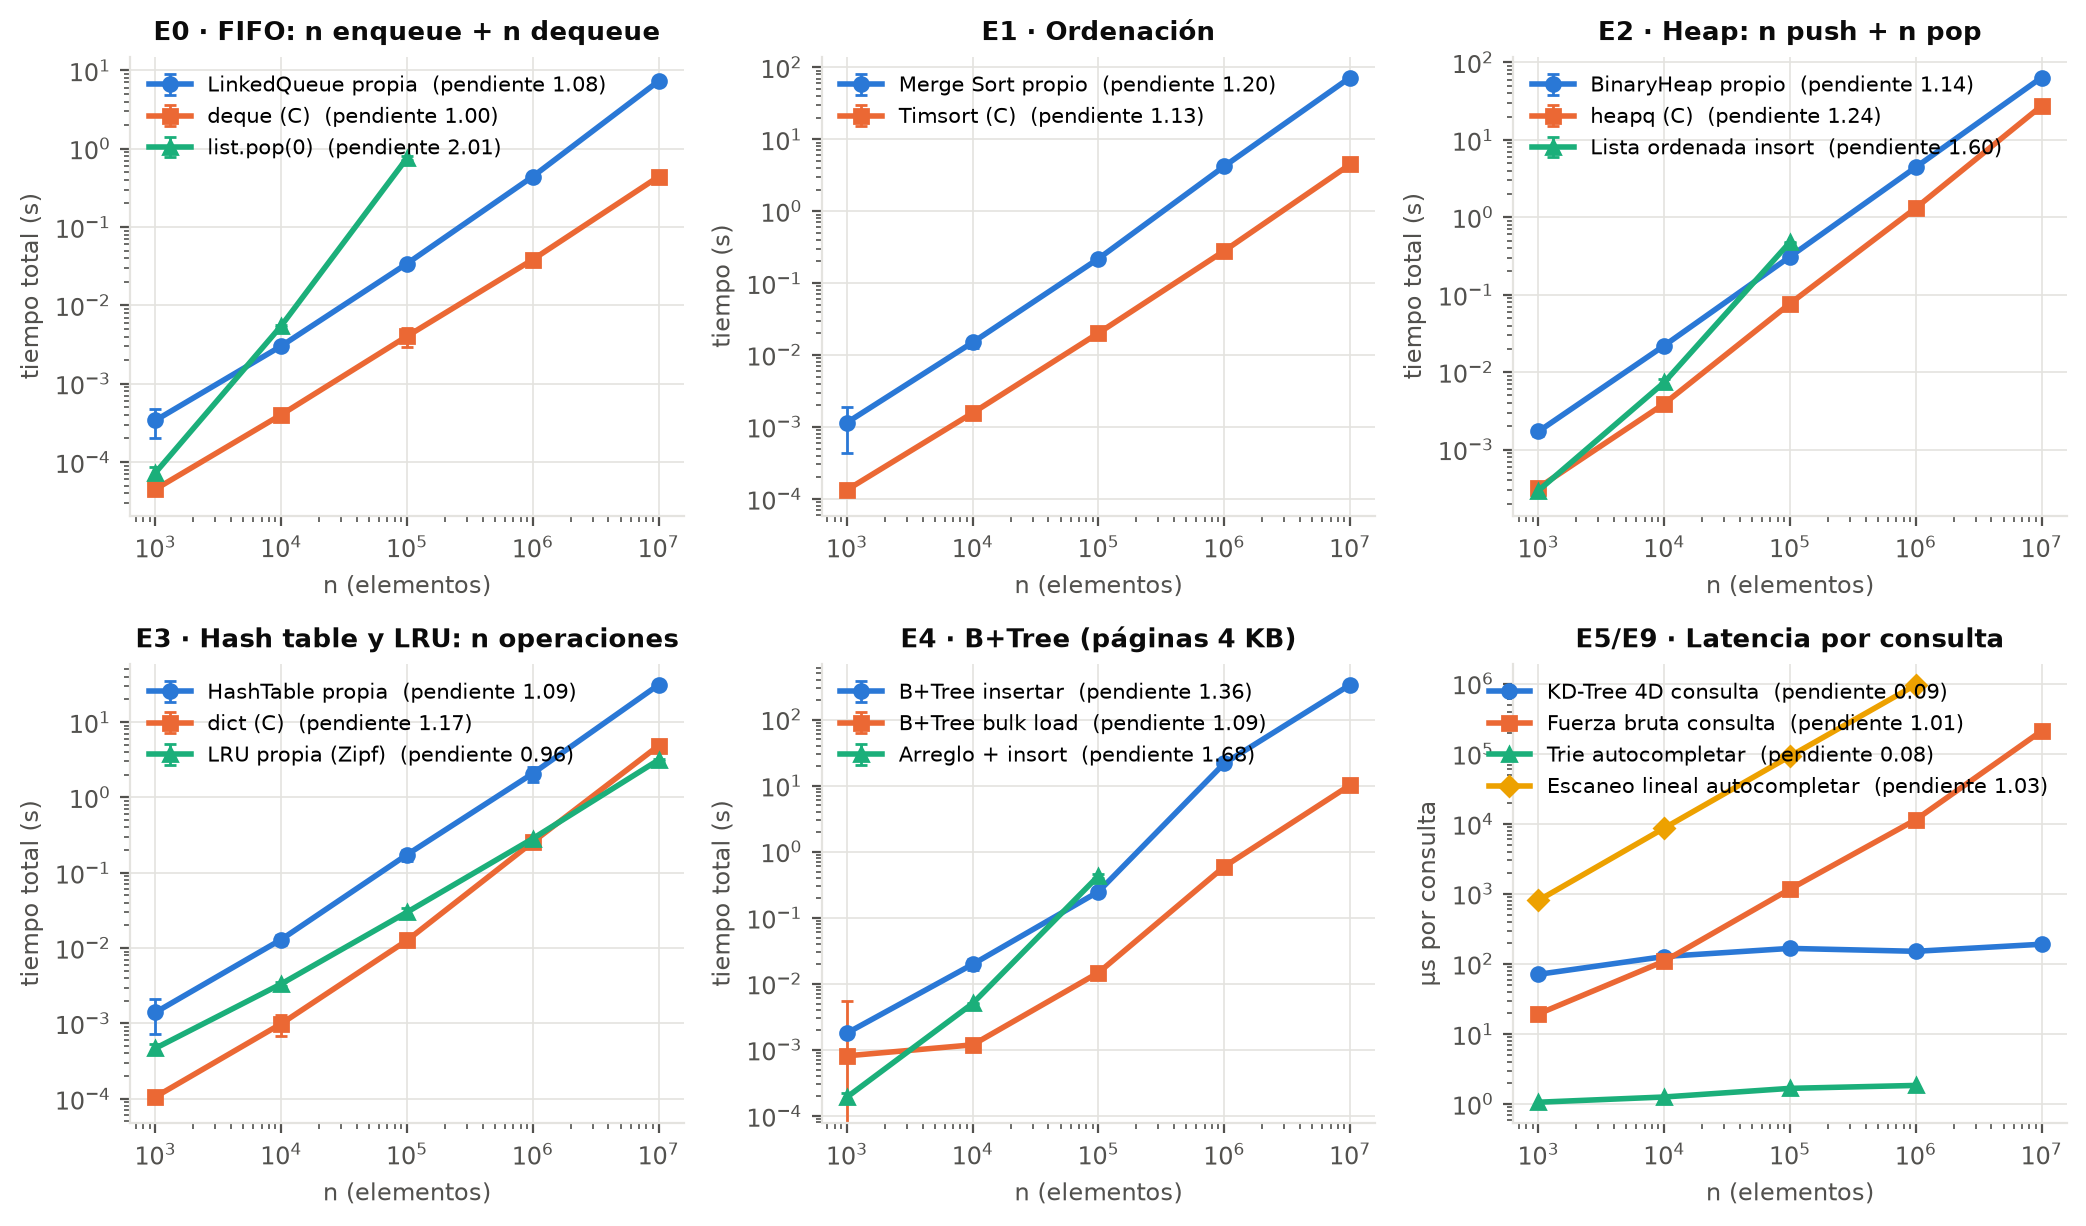
\includegraphics[width=\linewidth]{../../experiments/figures/fig_base_loglog.png}
\caption{Escalabilidad log-log (media $\pm$ desviación estándar) de las estructuras base frente a referencias en C y alternativas ingenuas; en la leyenda, la pendiente
ajustada $b$ de $t\propto n^b$ entre $10^3$ y el mayor tamaño medido ($10^7$ salvo las alternativas cuadráticas y el Trie).}\label{fig:base}
\end{figure}
\begin{table}[H]\centering
\caption{Pendiente ajustada $b$ ($t\propto n^b$, de $10^3$ al mayor tamaño medido) frente a la esperada; para latencias por consulta, $b\approx0$ indica costo sublineal.}\label{tab:slopes}
\setlength{\tabcolsep}{3.5pt}\footnotesize
\begin{tabular}{@{}lrl|lrl@{}}\toprule
Estructura / operación & $b$ & Esperada & Estructura / operación & $b$ & Esperada \\\midrule
LinkedQueue propia & 1.08 & 1 & Escaneo lineal autocompletar & 1.03 & 1 \\
deque (C) & 1.00 & 1 & Bloom insertar & 1.00 & 1 \\
list.pop(0) & 2.01 & 2 & set insertar & 1.13 & 1 \\
Merge Sort propio & 1.21 & $\approx$1.05-1.1 & Bloom consultar 2n & 1.01 & 1 \\
Timsort (C) & 1.13 & $\approx$1.05-1.1 & set consultar 2n & 1.15 & 1 \\
BinaryHeap propio & 1.15 & $\approx$1.05-1.1 & MinHash+LSH consulta & 0.06 & $\approx$0 \\
heapq (C) & 1.24 & $\approx$1.05-1.1 & Fuerza bruta Jaccard & 1.12 & 1 \\
Lista ordenada insort & 1.60 & 2 & HNSW consulta (ef=50) & 0.11 & $\approx$0 \\
HashTable propia & 1.09 & 1 & KNN exacto fuerza bruta & 1.06 & 1 \\
dict (C) & 1.17 & 1 & KD-Tree 32D & 0.95 & $\approx$1 \\
LRU propia (Zipf) & 0.96 & 1 & MinHash+LSH construir & 1.12 & 1 \\
B+Tree insertar & 1.36 & $\approx$1.05-1.1 & HNSW construir & 1.04 & $\approx$1.1 \\
B+Tree bulk load & 1.09 & 1 & PageRank & 1.07 & 1 \\
Arreglo + insort & 1.68 & 2 & Louvain & 1.22 & $\approx$1-1.2 \\
KD-Tree 4D consulta & 0.09 & $\approx$0-0.3 & Label Propagation & 1.22 & $\approx$1 \\
Fuerza bruta consulta & 1.01 & 1 & Grado ponderado & 0.51 & 0-1 \\
Trie autocompletar & 0.08 & 0 & & & \\
\bottomrule\end{tabular}
\end{table}
\vspace{-6pt}
Las pendientes confirman las complejidades esperadas (Tabla~\ref{tab:slopes}): FIFO propia 1.08 frente a 2.01 de \texttt{list.pop(0)}; Merge Sort 1.21 y heap 1.15
($n\log n$; algo por encima del 1.1 ideal por efectos de caché y asignación de memoria en $10^7$); tabla hash 1.09 (\Oh{1} por operación, 1.3–1.4 sondeos por operación con carga $\le$0.7); B+Tree \emph{bulk load} 1.09 (lineal) frente a 1.68 del
arreglo ordenado con \texttt{insort} (cuadrático por desplazamientos). El B+Tree con inserciones aleatorias tiene pendiente 1.36 porque desde $10^6$ claves
(7\,418 páginas) el árbol ya no cabe en el \emph{buffer pool} de 1\,024 páginas: cada inserción paga lecturas y escrituras de página reales (9.4M escrituras con
$10^7$ claves). Aun así, con $10^7$ claves la altura es 4 y una búsqueda puntual cuesta 1.7 lecturas de disco y 23\,µs; un rango de 10\,000 claves, 1.7\,ms. El
KD-Tree 4D responde KNN exacto en 0.15–0.19\,ms visitando 68–94 nodos tanto con $10^6$ como con $10^7$ puntos (pendiente 0.09), frente a 11\,ms y 211\,ms de la
fuerza bruta (1\,100$\times$ en $10^7$). El Trie responde autocompletado en 1–1.8\,µs independientemente de $n$ (pendiente 0.08) frente a 963\,ms del escaneo lineal con $10^6$ nombres.
Las referencias en C son 3–15$\times$ más rápidas en tiempo constante, como se espera de Python interpretado; la forma de las curvas es la misma.
\emph{Memoria pico} con $10^7$: FIFO 457\,MB, heap 1.29\,GB (tuplas), tabla hash 256\,MB (frente a 320\,MB de \texttt{dict}), KD-Tree 309\,MB y B+Tree 14\,MB en RAM
(282\,MB de páginas en disco). Límite: el Trie con $10^6$ nombres ocupa 1.7\,GB (4.3M nodos con su top-$K$ cacheado), por lo que $10^7$ nombres
($\approx$17\,GB) no cabe en 7.8\,GB y no se ejecutó; un catálogo real de comercio electrónico rara vez supera $10^6$ productos, y la alternativa sería un trie
comprimido (radix) o un FST.

\subsection{Filtrado probabilístico (E6)}
\begin{figure}[H]\centering
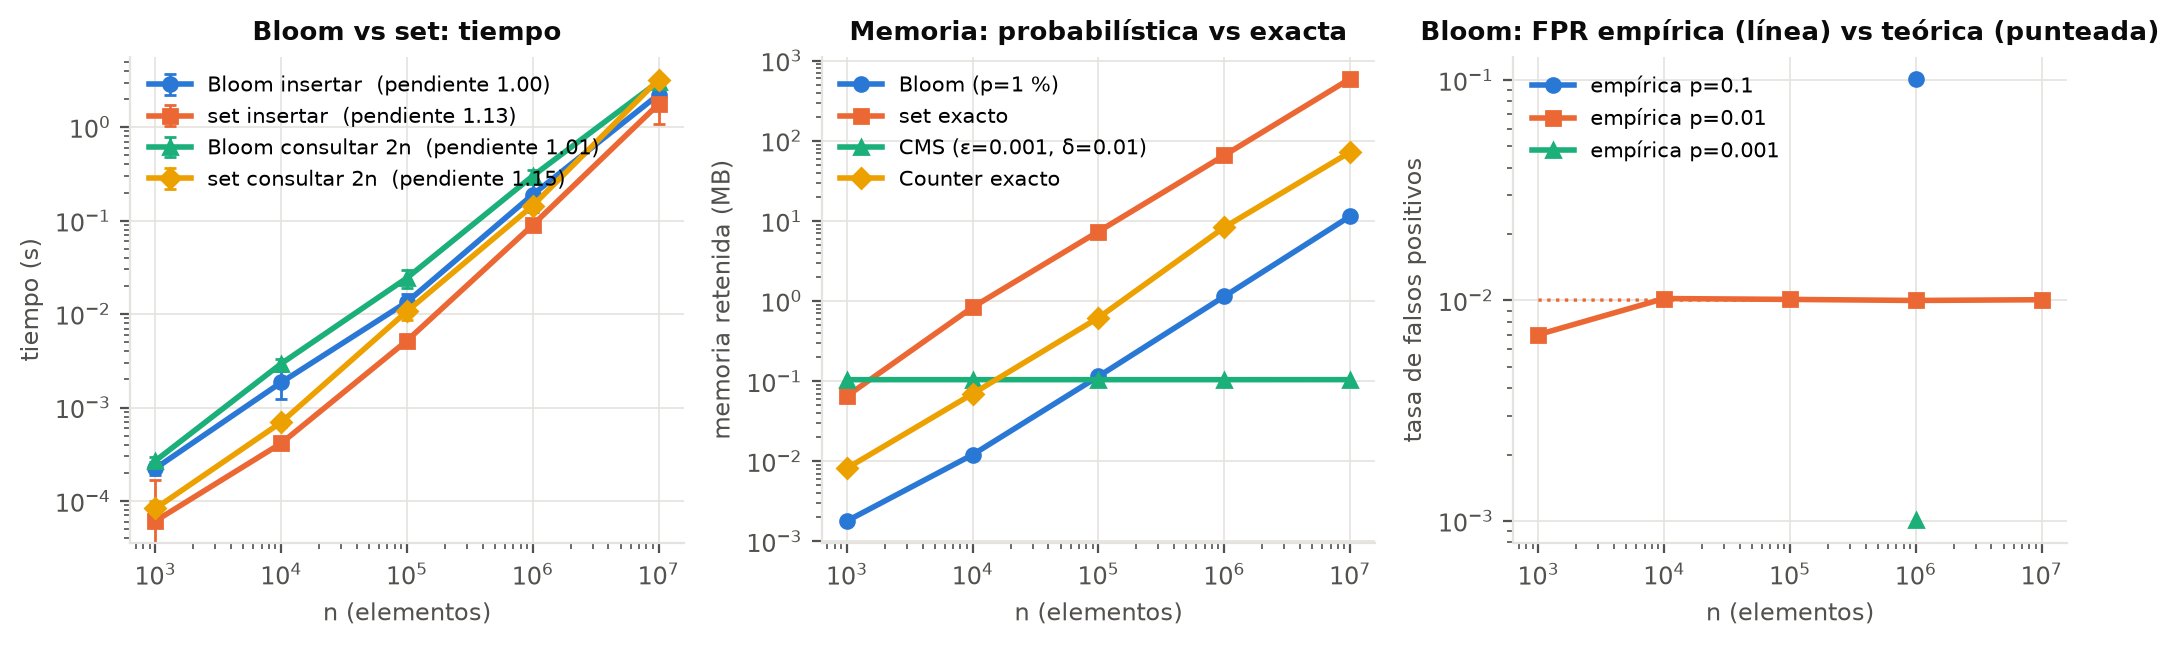
\includegraphics[width=\linewidth]{../../experiments/figures/fig_probabilisticas.png}
\caption{Bloom Filter frente a \texttt{set} (tiempo y memoria), CMS frente a \texttt{Counter} (memoria) y FPR empírica del Bloom frente a la teórica.}\label{fig:prob}
\end{figure}
\vspace{-6pt}
\begin{table}[H]\centering\small
\caption{Estructuras probabilísticas frente a la alternativa exacta (memoria retenida medida con tracemalloc; RSS en $10^7$).}\label{tab:prob}
\resizebox{\linewidth}{!}{\setlength{\tabcolsep}{4pt}
\begin{tabular}{@{}llllll@{}}\toprule
Comparación & $n$ & Construir (aprox./exacto) & Consultar $2n$ & Memoria (aprox./exacto) & Calidad \\\midrule
Bloom ($p$=1\,\%) vs \texttt{set} & $10^5$ & 13.46 ms / 5.19 ms & 24.36 ms / 10.71 ms & 118 KB / 7.4 MB & FPR 1.011\,\% (teórica 1.004\,\%), FN = 0 \\
Bloom ($p$=1\,\%) vs \texttt{set} & $10^6$ & 189.92 ms / 89.68 ms & 300.52 ms / 144.64 ms & 1.1 MB / 65.8 MB & FPR 1.000\,\% (teórica 1.004\,\%), FN = 0 \\
Bloom ($p$=1\,\%) vs \texttt{set} & $10^7$ & 2.23 s / 1.77 s & 3.08 s / 3.24 s & 11.4 MB / 594.4 MB & FPR 1.008\,\% (teórica 1.004\,\%), FN = 0 \\
CMS ($\varepsilon$=0.001) vs \texttt{Counter} & $10^5$ & 4.34 ms / 6.60 ms & -- & 107 KB / 635 KB & err. medio 8, máx 35 ($\varepsilon N$=100); 100\,\% en cota; subestim. 0 \\
CMS ($\varepsilon$=0.001) vs \texttt{Counter} & $10^6$ & 57.39 ms / 122.94 ms & -- & 107 KB / 8.3 MB & err. medio 138, máx 380 ($\varepsilon N$=1000); 100\,\% en cota; subestim. 0 \\
CMS ($\varepsilon$=0.001) vs \texttt{Counter} & $10^7$ & 654.48 ms / 2.05 s & -- & 107 KB / 72.3 MB & err. medio 1505, máx 40991 ($\varepsilon N$=9997); 100\,\% en cota; subestim. 0 \\
\bottomrule\end{tabular}}
\end{table}
\vspace{-6pt}
El Bloom Filter cumple la FPR teórica en todos los tamaños (1.008\,\% medida frente a 1.004\,\% teórica con $10^7$ claves; 0.101\,\% frente a 0.100\,\% con $p=0.1\,\%$) y
nunca da falsos negativos, con 9.6 bits por elemento: \textbf{11\,MB frente a 594\,MB} del \texttt{set} exacto con $10^7$ claves (52$\times$ menos). El tiempo es del mismo
orden que el del \texttt{set} (ambos lineales; el \texttt{set} es C nativo), así que la ventaja del Bloom es de \textbf{memoria}, no de velocidad, y por eso se usa como
filtro frente a la verificación exacta. El CMS ocupa 104\,KB constantes ($w=2\,719$, $d=5$) frente a 72\,MB del \texttt{Counter} con $\sim$950\,000 claves distintas;
nunca subestimó y el 100\,\% de las estimaciones quedó dentro de la cota $\varepsilon N$. El precio es el error aditivo: con $N=10^7$ el error medio es 1\,505 y el
error relativo en los 100 más frecuentes es 12\,\%; en el pipeline la ventana de 5 minutos mantiene $N$ pequeño y el error es despreciable frente al umbral de 15.

\subsection{Similitud aproximada (E7)}
\begin{figure}[H]\centering
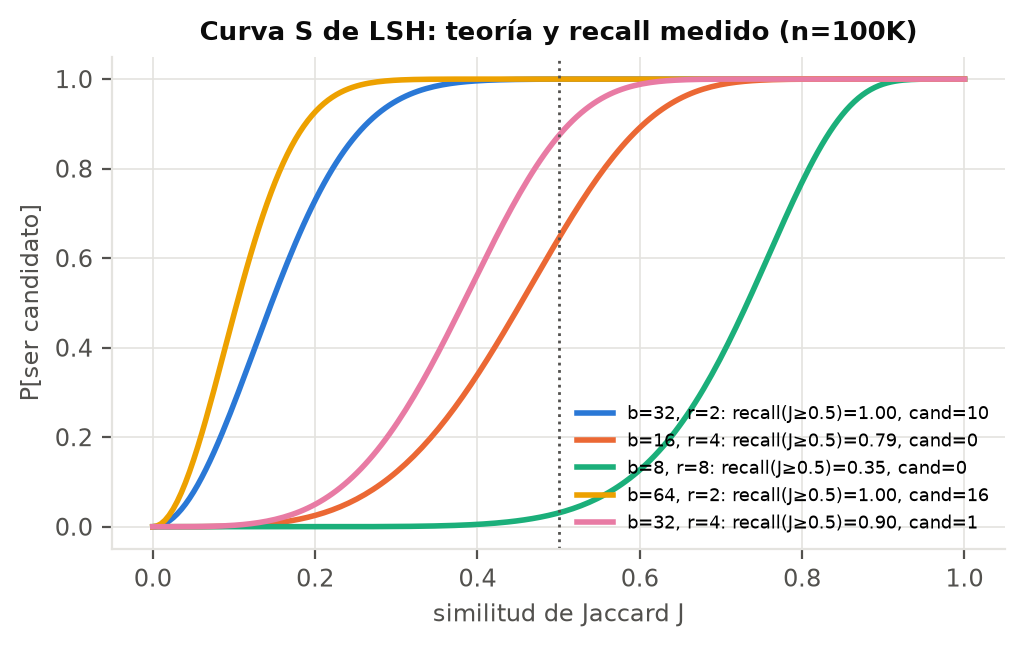
\includegraphics[width=0.36\linewidth]{../../experiments/figures/fig_lsh_curva.png}\hfill
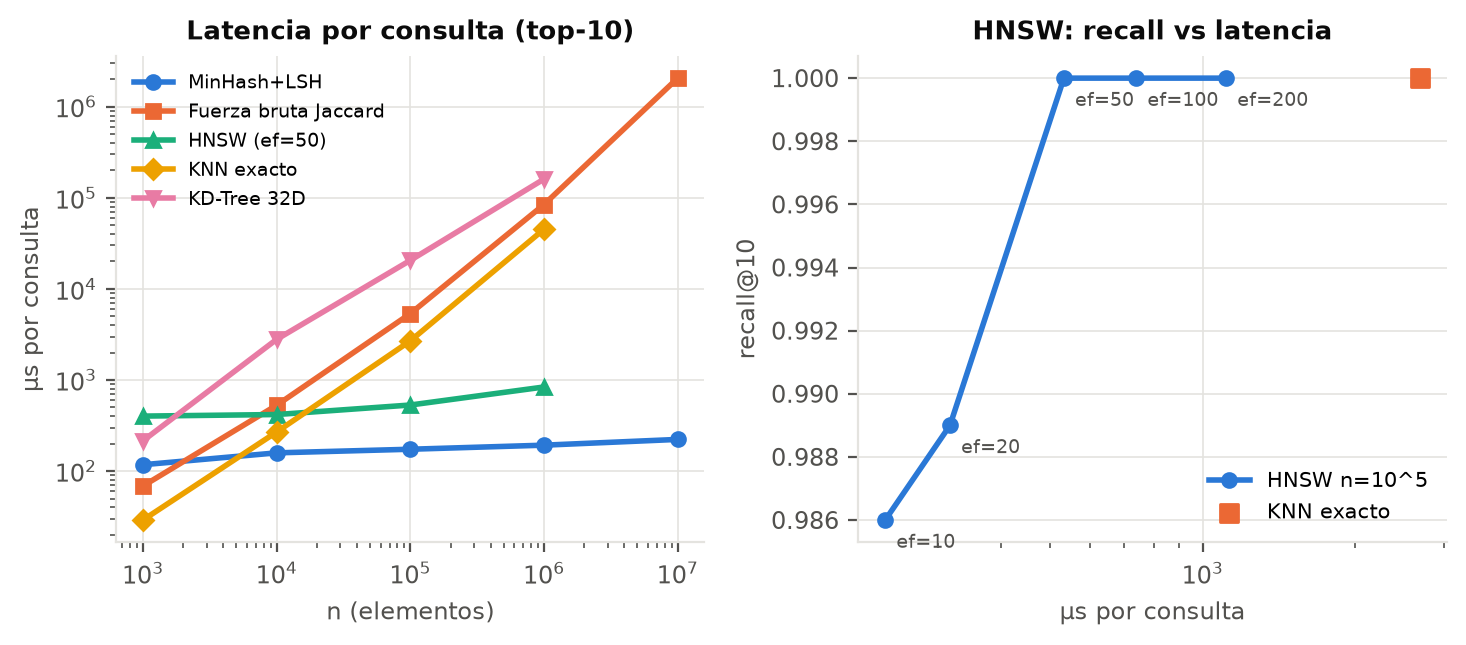
\includegraphics[width=0.63\linewidth]{../../experiments/figures/fig_similitud_ab.png}
\caption{Izquierda: curvas S teóricas de LSH y recall medido para varias $(b,r)$. Centro: latencia por consulta frente a $n$. Derecha: HNSW, recall@10 frente a latencia al variar $ef$ ($n=10^5$).}\label{fig:lsh}\label{fig:sim}
\end{figure}
\vspace{-6pt}
\begin{table}[H]\centering\small
\caption{Técnicas aproximadas frente a fuerza bruta / KNN exacto (consultas top-10).}\label{tab:sim}
\resizebox{\linewidth}{!}{\setlength{\tabcolsep}{4pt}
\begin{tabular}{@{}llrrrlll@{}}\toprule
Técnica & $n$ & Consulta aprox. & Exacto & Aceleración & Recall & Memoria (índice/datos) & Construcción \\\midrule
MinHash+LSH (32$\times$2) & $10^4$ & 0.16 ms & 0.5 ms & 3$\times$ & 1.00 (J$\ge$0.5) & 3.7 MB / 471 KB & 117.39 ms \\
MinHash+LSH (32$\times$2) & $10^5$ & 0.17 ms & 5.4 ms & 31$\times$ & 1.00 (J$\ge$0.5) & 36.6 MB / 4.6 MB & 2.77 s \\
MinHash+LSH (32$\times$2) & $10^6$ & 0.19 ms & 84.4 ms & 438$\times$ & 1.00 (J$\ge$0.5) & 366.2 MB / 45.8 MB & 30.64 s \\
MinHash+LSH (32$\times$2) & $10^7$ & 0.22 ms & 2\,057.7 ms & 9\,231$\times$ & 1.00 (J$\ge$0.5) & 2.40 GB / 457.8 MB & 232.62 s \\
HNSW ($M$=16, $ef$=50) & $10^4$ & 0.42 ms & 0.3 ms & 0.6$\times$ & 1.000 (@10) & 4.7 MB / 1.2 MB & 29.08 s \\
HNSW ($M$=16, $ef$=50) & $10^5$ & 0.53 ms & 2.7 ms & 5.1$\times$ & 1.000 (@10) & 48.9 MB / 12.2 MB & 296.74 s \\
HNSW ($M$=16, $ef$=50) & $10^6$ & 0.84 ms & 45.2 ms & 53.9$\times$ & 0.989 (@10) & 321.4 MB / 122.1 MB & 3324.31 s \\
\bottomrule\end{tabular}}
\end{table}
\vspace{-6pt}
\textbf{MinHash+LSH.} La consulta cuesta $\sim$0.2\,ms casi constante (pendiente 0.06) porque compara solo $\sim$10 candidatos; la fuerza bruta crece linealmente
(84\,ms en $10^6$ y 2.1\,s por consulta en $10^7$): \textbf{$\sim$9\,000$\times$ más rápido en $10^7$ con recall 1.0} para los vecinos con $J\ge0.5$. El recall sobre el top-10 completo
es 0.15–0.25 porque, más allá de los casi-duplicados, los vecinos tienen $J\approx0$ y LSH está diseñado para no verlos. El costo es la memoria: el índice ocupa
2.4\,GB frente a 458\,MB de los conjuntos en $10^7$ y se construye en 233\,s. La curva S (Fig.~\ref{fig:lsh}) muestra el compromiso: $16\times4$ (umbral 0.5) pierde 21\,\%
de los vecinos con $J\ge0.5$; $8\times8$, el 65\,\%; $32\times2$ los recupera todos con 10 candidatos y $64\times2$ con 16.
\textbf{HNSW.} Con $10^6$ vectores de 32 dimensiones responde en 0.84\,ms con recall@10 = 0.989, frente a 45\,ms del KNN exacto (54$\times$); con $10^5$, $ef=10$ da 0.986
en 0.24\,ms y $ef\ge50$ da recall 1.0. La construcción es el cuello de botella en Python (2.5–3.3\,ms por inserción; 55 minutos para $10^6$): con $10^7$ serían
$\sim$10 horas, por lo que el experimento de HNSW llega a $10^6$ (en C, \texttt{hnswlib} construye $10^7$ en minutos). El KD-Tree en 32D visita el 82\,\% de los nodos
y es más lento que la fuerza bruta (161\,ms frente a 45\,ms): evidencia directa de la maldición de la dimensionalidad que justifica usar KD-Tree solo en 4D (E5).

\subsection{Grafo: influencia y comunidades (E8)}
\begin{figure}[H]\centering
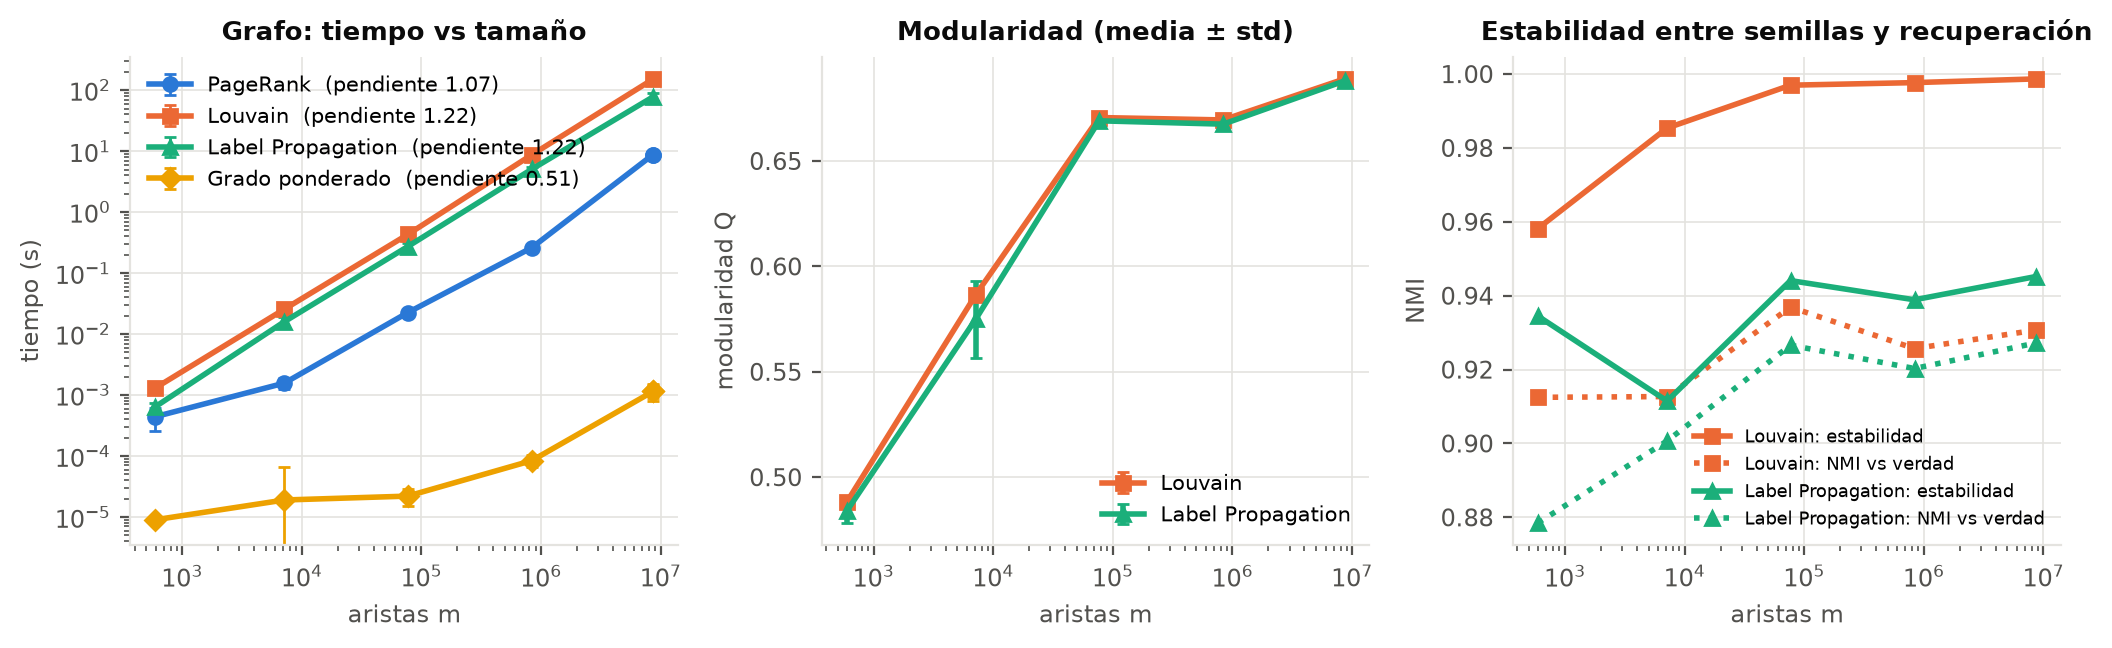
\includegraphics[width=\linewidth]{../../experiments/figures/fig_grafo.png}
\caption{Grafo con comunidades plantadas (70\,\% de aristas internas, grados Zipf, $n/8$ nodos): tiempo, modularidad (media $\pm$ std) y estabilidad/recuperación (NMI).}\label{fig:grafo}
\end{figure}
\vspace{-6pt}
\begin{table}[H]\centering\small
\caption{Louvain frente a Label Propagation en el mismo grafo (media sobre 10 semillas; 5 en $10^6$; 2 en $10^7$).}\label{tab:com}
\resizebox{\linewidth}{!}{\setlength{\tabcolsep}{4pt}
\begin{tabular}{@{}llllllll@{}}\toprule
Grafo ($n$ interacciones) & Alg. & Modularidad $Q$ & Tiempo & Nº comunidades & Mayor / mediana & Estabilidad (NMI) & NMI vs verdad \\\midrule
$10^4$ (7\,146 ar.) & Louvain & 0.5865 $\pm$ 0.0002 & 25.61 ms & 17 $\pm$ 0.0 & 310 / 54 & 0.985 & 0.913 \\
$10^4$ (7\,146 ar.) & LPA & 0.5750 $\pm$ 0.0183 & 15.96 ms & 19 $\pm$ 1.4 & 333 / 47 & 0.911 & 0.901 \\
$10^5$ (76\,778 ar.) & Louvain & 0.6706 $\pm$ 0.0000 & 429.72 ms & 56 $\pm$ 0.0 & 783 / 184 & 0.997 & 0.937 \\
$10^5$ (76\,778 ar.) & LPA & 0.6691 $\pm$ 0.0010 & 272.55 ms & 85 $\pm$ 2.2 & 805 / 133 & 0.944 & 0.927 \\
$10^6$ (835\,535 ar.) & Louvain & 0.6695 $\pm$ 0.0000 & 8.71 s & 167 $\pm$ 0.6 & 14\,491 / 431 & 0.998 & 0.926 \\
$10^6$ (835\,535 ar.) & LPA & 0.6675 $\pm$ 0.0005 & 5.05 s & 519 $\pm$ 12.7 & 15\,397 / 2 & 0.939 & 0.920 \\
$10^7$ (8\,641\,533 ar.) & Louvain & 0.6889 $\pm$ 0.0000 & 152.04 s & 553 $\pm$ 0.0 & 54\,995 / 1360 & 0.999 & 0.931 \\
$10^7$ (8\,641\,533 ar.) & LPA & 0.6880 $\pm$ 0.0000 & 77.88 s & 4\,722 $\pm$ 47.4 & 58\,061 / 2 & 0.945 & 0.927 \\
Co-compra real (15\,390 ar.) & Louvain & 0.7553 $\pm$ 0.0018 & 451.55 ms & 221 & 829 / 2 & 0.866 & -- \\
Co-compra real (15\,390 ar.) & LPA & 0.6303 $\pm$ 0.0111 & 190.62 ms & 848 & 372 / 3 & 0.860 & -- \\
\bottomrule\end{tabular}}
\end{table}
\vspace{-6pt}
\textbf{PageRank} converge en 38–42 iteraciones con costo lineal en $m$ (pendiente 1.07; 8.6\,s con 8.6M aristas). En un grafo no dirigido su correlación con el grado es
alta (Spearman 0.985; 95–99\,\% de coincidencia en el top-100), por lo que su valor diferencial está en la versión \textbf{personalizada}, que el ranking por grado no puede
dar: PPR desde el carrito es la señal con mayor peso del recomendador. \textbf{Comunidades:} en el grafo sintético ambos algoritmos alcanzan modularidades parecidas, pero
Louvain es \textbf{casi determinista} (NMI entre semillas 0.985–0.999 frente a 0.91–0.945; desviación de $Q\le2\cdot10^{-4}$ frente a hasta $2\cdot10^{-2}$ en LPA) y \textbf{no fragmenta}:
LPA deja miles de comunidades diminutas (mediana 2 nodos, 4\,722 comunidades en $10^7$ frente a 553). LPA es $\sim$2$\times$ más rápido. En el grafo de co-compra
\emph{real} del pipeline (1M eventos, 5\,681 productos, 15\,390 aristas), la diferencia es clara: Louvain $Q=0.755\pm0.002$ con 221 comunidades frente a LPA
$Q=0.630\pm0.011$ con 848; las comunidades de Louvain agrupan categorías complementarias plantadas (en la demo, la mayor reúne 91 laptops con 43 mouse, 42 teclados y 26 monitores).
